\section{Approach}\label{sec:approach}

In this section, we describe our algorithm for assignee prediction. We consider bug triage as a ranking problem, which we believe to be more appropriate here, because it does not depend on the current set of developers. The classifying setting requires an immutable set of predicted classes. If a developer leaves the project, they should be filtered out of the resulting prediction afterwards, and when a new developer joins, the classifying model will have to be retrained to take them into account. Since developers in the project may come and go, a more suitable option is the ranking problem setting, in which it is necessary to evaluate the relevance function $f(q, d)$ for a bug $q$ and a developer $d$.

More formally, given a query $q$ (bug) and a collection $D$ of documents (developers) that match the query, the task is to find a function $f$ such that $(q, d) \prec (q, d') \Leftrightarrow f(q, d) < f(q, d')$, where $(q, d) \prec (q, d')$ means that $d$ has a rank lower than $d'$. Function $f$ maps query-documents pairs to a relevance score.

The proposed model uses bug stack traces as the primary source of information for predicting assignees. In order to obtain better results, we also build features from the version control system (VCS) annotations, which provide information on which developer modified each line of the file and when. For example, Git annotations can be obtained via the \textit{git blame} or \textit{git annotate} commands.

The overall pipeline of the proposed algorithm is presented in \Cref{fig:approach-architecture}. Using deep learning methods, the bug and the developer are mapped to a vector of a fixed size (embedding). We transform each bug stack trace into a sequence of text tokens (\Cref{sec:preprocessing}) and apply the ideas from text sequences processing to obtain embeddings of bugs (\Cref{sec:vector-representation}). Then, to create an embedding of a developer, we process all the files in the given stack trace to find files that the developer edited, and use this information to map this developer into the stack trace embedding space (\cref{sec:dev-representation}). After all the embeddings are extracted, they are compared using the comparison module (\Cref{sec:vector-similarity}), and the score is obtained, which shows the relevance of the bug and the developer. To get the most appropriate developers for a given bug, we simply have to rank all the developers by their score. 

\begin{figure}[t]
    \centering
    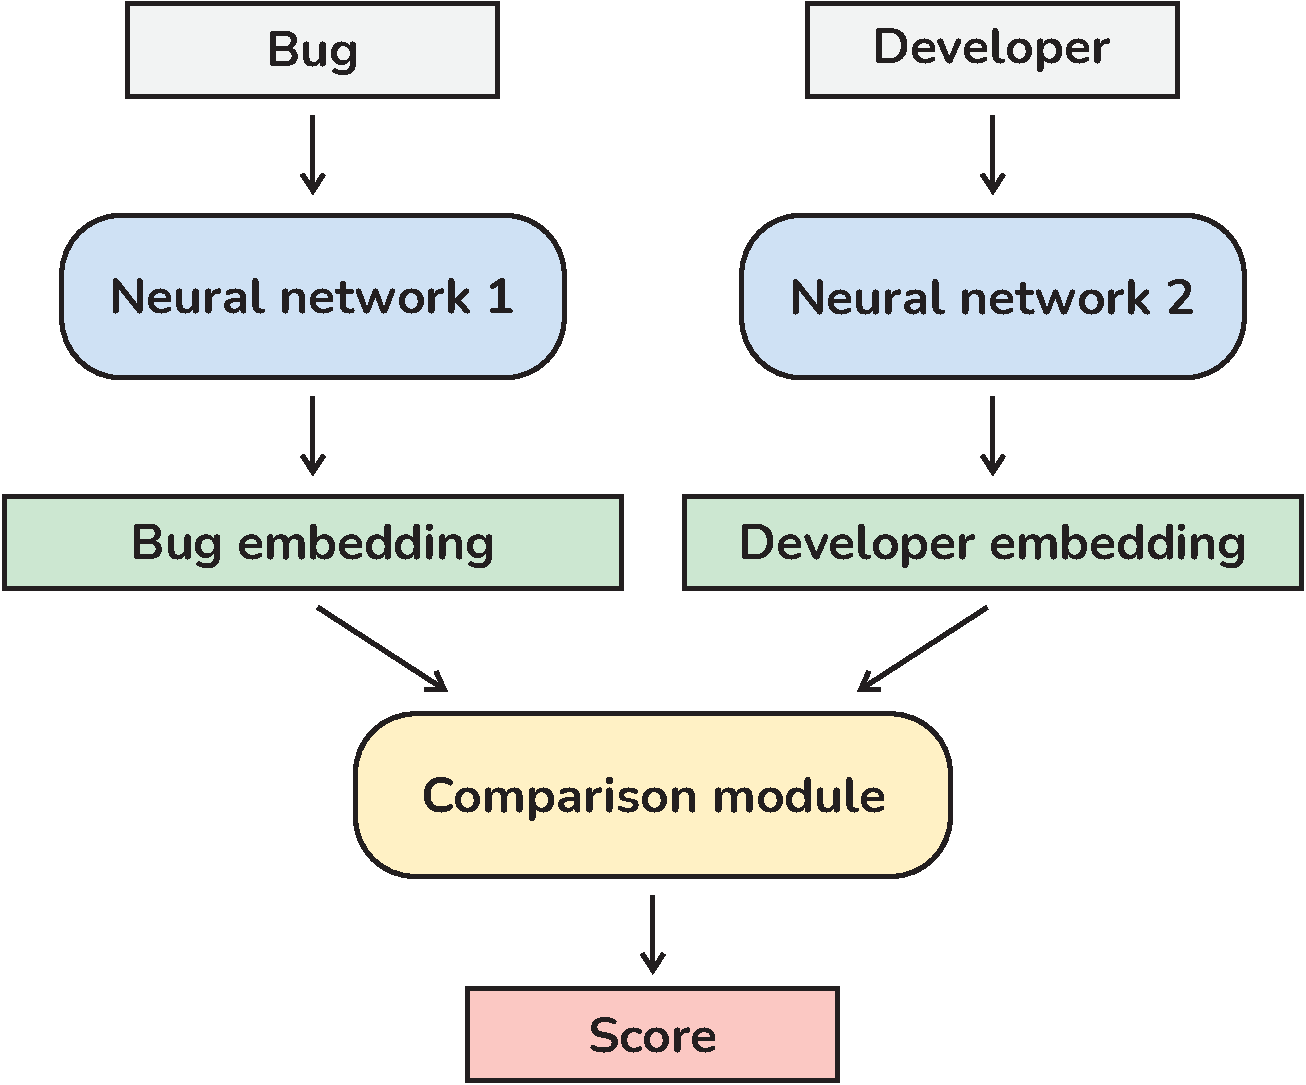
\includegraphics[width=0.7\columnwidth]{figures/03-approach/architecture.pdf}
    \centering
    \caption{The overall pipeline of the approach.}
    \label{fig:approach-architecture}
\end{figure}

To improve our model, we use additional features based on the VCS annotations and propose to process the annotations in two different ways: manually (\Cref{sec:manual-features}) and using an additional neural network (\Cref{sec:neural-features}) that allows us to avoid complex feature engineering. 
Let us now describe these steps in greater detail.

\secpart{Preprocessing}
\label{sec:preprocessing}

The stack trace is represented as a sequence of frames $ST = \{ f_1, f_2, \ldots, f_n \}$, where $f_i$ is the $i$-th stack frame. Every frame has a method name, a file name, a subsystem name, a commit hash, and an error line. An example of a stack frame is presented in~\Cref{fig:introduction-frame-example}.

Our preliminary experiments showed that stack trace preprocessing is an essential step that can significantly improve the model quality. In our work, we used the following data processing steps.

Firstly, we noticed that the length of the stack trace can sometimes be quite large. For instance, the maximum stack trace length in our dataset reached as many as 15,000 frames. It is difficult to make a neural network remember all the information as the frames are processed one by one. On the other hand, long stack traces tend to relate to a \textit{StackOverflowException} error. Oftentimes, such a stack trace contains a loop: a set of frames that repeat at a specific frequency. Replacing the loop with the first occurrence of the loop element allows us to significantly reduce the length of the trace stack without degrading the model's quality. We did this for every stack trace in the dataset where it is applicable.

Secondly, because of the way the dataset was collected, not all information is available for every frame, the frame fields can be null. If the text token received from the frame is null, then we skip this frame.

In order to apply existing approaches, we propose to represent a stack trace as a sequence of text tokens using the following technique. Firstly, we extract the method name, the file name, or the subsystem name from each frame of the stack trace. For example, the stack frame in \Cref{fig:introduction-frame-example} can be mapped to \textit{org.mockito.internal.MockitoCore.mockStatic}, \textit{MockitoCore.java}, or \textit{org.mockito.internal}, respectively. Thus, the stack trace will be presented as a sequence of text tokens, which can be processed with various deep learning approaches. We conducted experiments with all three options (method name, file name, or subsystem), and since the difference was insignificant, we decided to extract the stack trace file name.

\secpart{Representing Stack Traces as Vectors}
\label{sec:vector-representation}

To represent a stack trace with a vector of a fixed length (\textit{i.e.}, embedding), we were inspired by the architectures applied in the previous works, namely, RNNs with attention and CNNs~\cite{Lee2017ApplyingDL, Guo2020DeveloperAM, Zaidi2020ApplyingCN, Mani2019DeepTriageET}. These two types of neural networks are among the most popular in the natural language processing field. In our study, we experimented with both of them.

\subsecpart{Recurrent Neural Network}

An RNN architecture called LSTM~\cite{Hochreiter1997LongSM} is frequently used to handle sequential data. It takes a sequence of text tokens as input and produces the resulting vectors. However, LSTMs may have problems remembering long sequences~\cite{Vaswani2017AttentionIA}, which can be fixed with a bidirectional network~\cite{Graves2005BidirectionalLN} with attention. The attention technique allows to focus on important parts of the input data~\cite{Bahdanau2015NeuralMT}. For instance, frames that are at the top of the stack trace are usually more informative and useful. 

We use the neural network architecture from the work of Maini et al.~\cite{Mani2019DeepTriageET}. The input of the model is a sequence of vector representations of words, $\mathbf{x} = \{ \mathbf{x_1}, \mathbf{x_2}, \ldots, \mathbf{x_n} \}$. In our approach, we use trainable embeddings for every text token. The network is bidirectional, therefore, the sequence is processed in both directions. The RNN produces a sequence of outputs $\mathbf{y} = \{\mathbf{y_1}, \mathbf{y_2}, \ldots, \mathbf{y_n} \}$ from each direction. After that, the attention mechanism is applied, which is the weighted sum of the RNN outputs:
\begin{align}
    \mathbf{a_n} = \sum_{i = 1}^{n} \alpha_i \mathbf{y_i},
\end{align}
where $\alpha_i$ represents an attention weight for the $i$-th output vector. 


The final representation $\mathbf{r}$ is obtained as follows:
\begin{align}
    \mathbf{r} = \underbrace{\mathbf{y_n} \oplus \mathbf{a_n}}_\text{forward LSTM} \oplus \underbrace{\mathbf{y_n} \oplus \mathbf{a_n}}_\text{backward LSTM},
\end{align}
where $\oplus$ represents the concatenation of vectors. It is easy to see that if the output vector has dimension $d$, then the embedding $r$ will be of size $4 \times d$.

\subsecpart{Convolutional Neural Network}

Another possible approach to represent a stack trace with a vector is to use CNN. CNNs are most commonly applied to analyze visual information, however, they can also solve natural language processing tasks~\cite{Collobert2008AUA}.

In a CNN-based network, for each sequence of text tokens, we build a matrix $\mathbf{S} \in \mathbb{R}^{s \times d}$, where $s$ is the sequence length and $d$ is the embedding dimension. We were inspired by the work of Lee et al.~\cite{Lee2017ApplyingDL} when building the model architecture. Similarly to them, we use trainable embeddings for text tokens. After that, a convolution layer with 1D convolutions is used to extract different patterns from the sequence of tokens. After applying each convolution filter, a feature vector is obtained. In the extracted feature vector, the subsampling process called max-pooling is applied, which is the operation of extracting the maximum element from a vector. The final representation $\mathbf{r}$ is obtained by concatenating max-pooling values and has a dimension equal to the total number of convolutions.

\secpart{Representing Developers as Vectors}
\label{sec:dev-representation}
Obtaining an embedding of a given bug is pretty straightforward, since each bug has a stack trace that can be transformed into a sequence of text tokens. However, the process of extracting the embedding of a developer is not that obvious. 

One possible solution is to represent the developer as all the code they wrote in the system. This approach has a significant drawback: the need to regularly re-index a large amount of data. If the developer has written new code in the system, then this must be taken into account. Continuous and efficient updates of the developer's embedding is a challenging task. 

To address this problem, we propose to map every developer to a specific synthetic stack trace, more specifically, a sequence of stack frames that they edited. In order not to deal with large-scale re-indexing, we do not use all the available stack traces, but only the stack trace of the current (query) bug. This way, the developer embedding will be bug-dependent: different vector representations are built for different errors, there is no single developer representation. This approach allows us to build the embedding of a developer much faster. The average length of a stack trace in our datasets is 50 frames, therefore, it is enough to look at about 50 files in order to map the developer to their stack trace. Furthermore, the resulting ``developer stack trace'' can be handled in the exact same way as the bug stack trace, and it is possible to use the same network architecture for the bug and for the developer, because each of them is represented in the same form. 

\Cref{alg:developer-stacktrace} shows the pseudo-code for the building of this developer stack trace. In this algorithm, we look at all frames from the stack trace of the current bug from first to last. If the developer has edited at least one line from the file of the given frame, then this frame is included in the developer stack trace. Each stack trace is an ordered sequence of frames, they are numbered starting from the top of the stack. While building the developer stack trace, the order of the frames is preserved. The order of the frames is significant, because generally frames at the top of the stack are more revealing.

\begin{algorithm}
    \caption{The building of the developer stack trace.}\label{alg:developer-stacktrace}
        \begin{algorithmic}
            \Input Developer $dev$, stack trace $stack$
            \Output Developer stack trace $dev\_stack$
            \State dev\_stack $\gets$ emptyList
            
            \For{frame in stack}
                \State file $\gets$ getFrameFile(frame)
                \State authors $\gets$ getFileAuthors(file)
                
                \If{dev $\in$ authors}
                    dev\_stack.append(frame) 
                \EndIf
                
            \EndFor
            \Return dev\_stack
        \end{algorithmic}
\end{algorithm}

It is important to note that the inner frames in the stack trace can include files from various libraries, in which case they will not have been edited by any of the developers in the project. We leave dealing with this case specifically for future work, for example, it might be possible to use the history of the developer's work to see whether they fixed bugs that relate to this particular library.

Overall, for each bug and each developer, we obtain a special stack trace that contains only the frames that concern files that this developer has edited. This allows us to compare the resulting embeddings.

\begin{table*}
    \centering
    \caption{Additional features obtained from the VCS annotations and their normalizations.}
    \label{table:annot-features}
    \begin{tabular}{cll}
        \toprule
        \multicolumn{1}{c}{\textbf{Category}} & 
        \multicolumn{1}{c}{\textbf{Description}} & \multicolumn{1}{c}{\textbf{Normalizations}} \\ 
        \midrule
        \multirow{8}{4em}{\textbf{Frame}} 
        & 
        Minimum distance from the edited line to the error line & Raw; annotation length; min \\
        & 
        Did the developer edit the error line? & Raw  \\
        & 
        Normalized number of edited lines in the file & Annotation length; max \\
        & 
        Normalized number of edited lines weighted by time & Annotation length; max \\ 
        & 
        Normalized number of edited lines in the window of size 10 & Window size; max \\
        & 
        Number of different developer's timestamps & Raw; max \\
        &
        Time passed since the last edit & Exp(-x); Log(x) \\ 
        & 
        Time passed since the first edit & Log(x) \\
        \midrule
        \multirow{5}{4em}{\textbf{Stack}} 
        & 
        The order of the first edited frame & Raw; stack length; number of annotated frames; min \\
        & 
        Normalized number of edited error lines & Stack length; max \\
        & 
        Normalized number of edited lines & Total number of lines; max \\
        &  
        Normalized number of edited lines in the frame with maximum IDF & Annotation length \\
        & 
        Normalized number of edited frames & Stack length; number of annotated frames; max \\
        \bottomrule
    \end{tabular}
\end{table*}

\secpart{Additional Features}
\label{sec:manual-features}

To improve the performance of the model, we enrich the embedding with the features built from the VCS annotations. 
The annotations provide information about who was the last person to have changed each line in the file, and when this change took place. The rationale behind using annotations is the following: if a developer has recently edited some file, it is more likely that their changes resulted in a bug. Therefore, such a developer should probably fix the current bug. 

An example of the first five lines of an annotation is shown in \Cref{fig:annotation-example}. Each developer is encoded with a unique identifier, and the time is represented in the Unix epoch format. 

\begin{figure}[htbp]
    \centering
    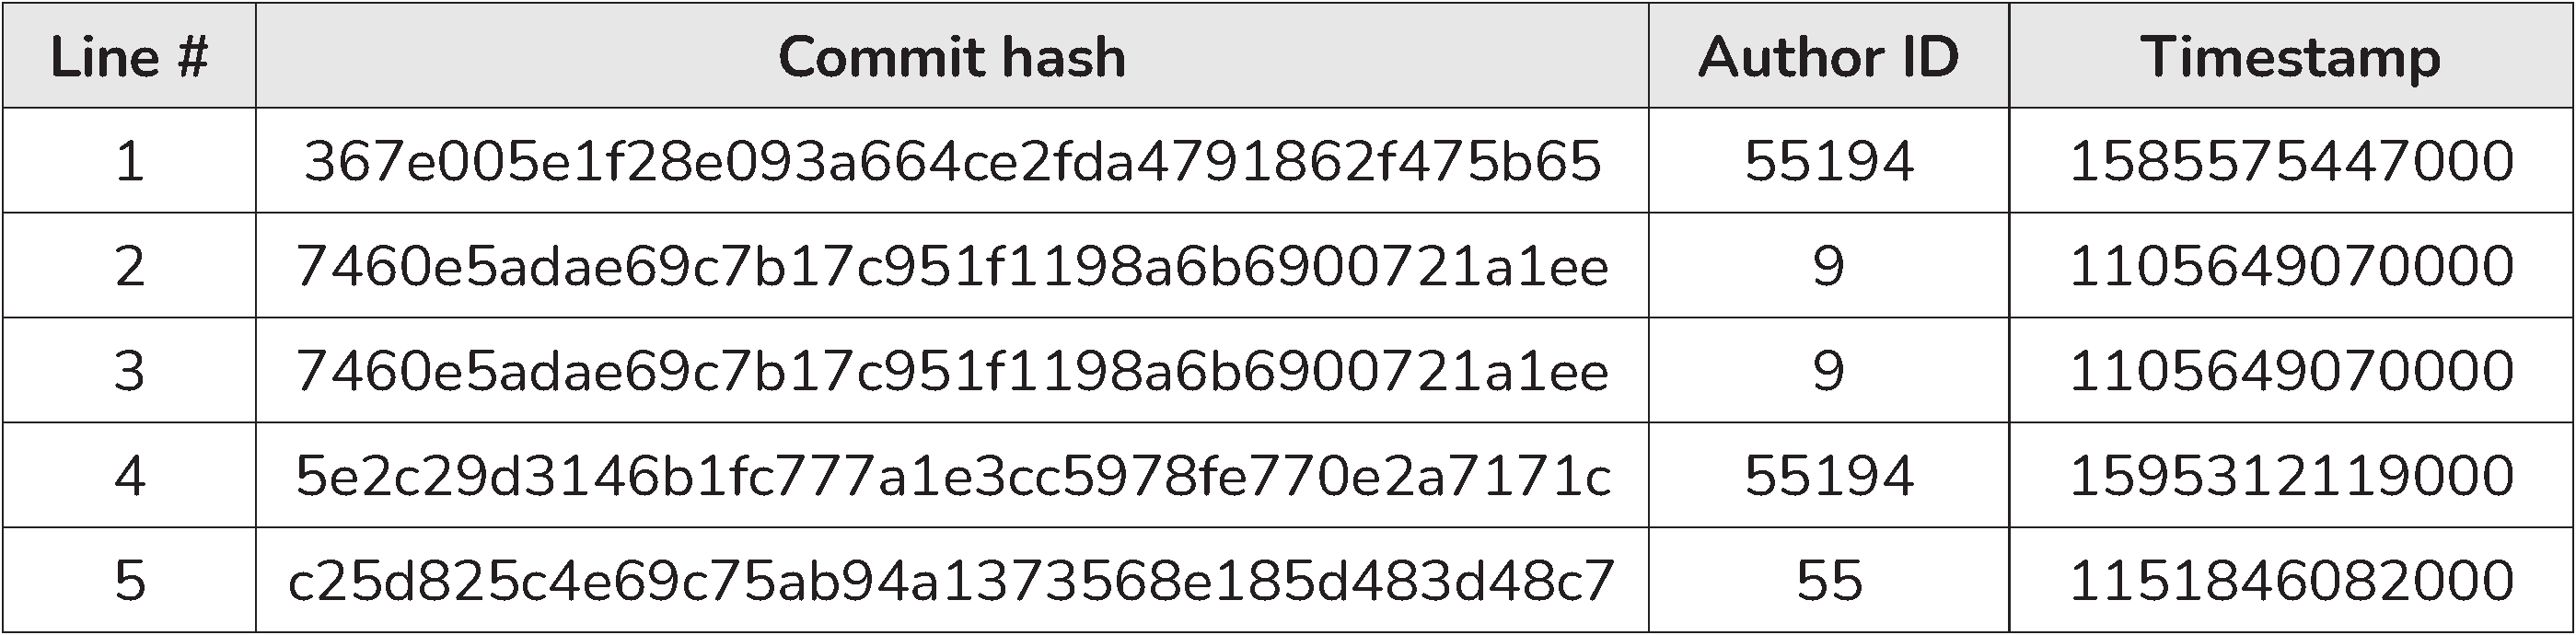
\includegraphics[width=\columnwidth]{figures/03-approach/annotation.pdf}
    \centering
    \vspace{-0.2cm}
    \caption{An example of the first lines of an annotation.}
    \label{fig:annotation-example}
\end{figure}

Additional features can be constructed both on the level of individual stack frame (\textit{e.g.}, how many lines in the file of a specific frame the developer edited) and on the level of the entire stack trace (\textit{e.g.}, how many stack frames have files that the developer edited), and are applied in different ways.

Features that relate to individual frames can be concatenated to the trainable embeddings before applying the RNN (\Cref{sec:vector-representation}). \Cref{fig:approach-frame-features} shows the proposed approach: a text token is extracted from the frame, each text token is associated with a trainable embedding, and the additional feature vector is concatenated to the embedding. The resulting vector becomes the input of the RNN.
    
    \begin{figure}[htbp]
        \centering
        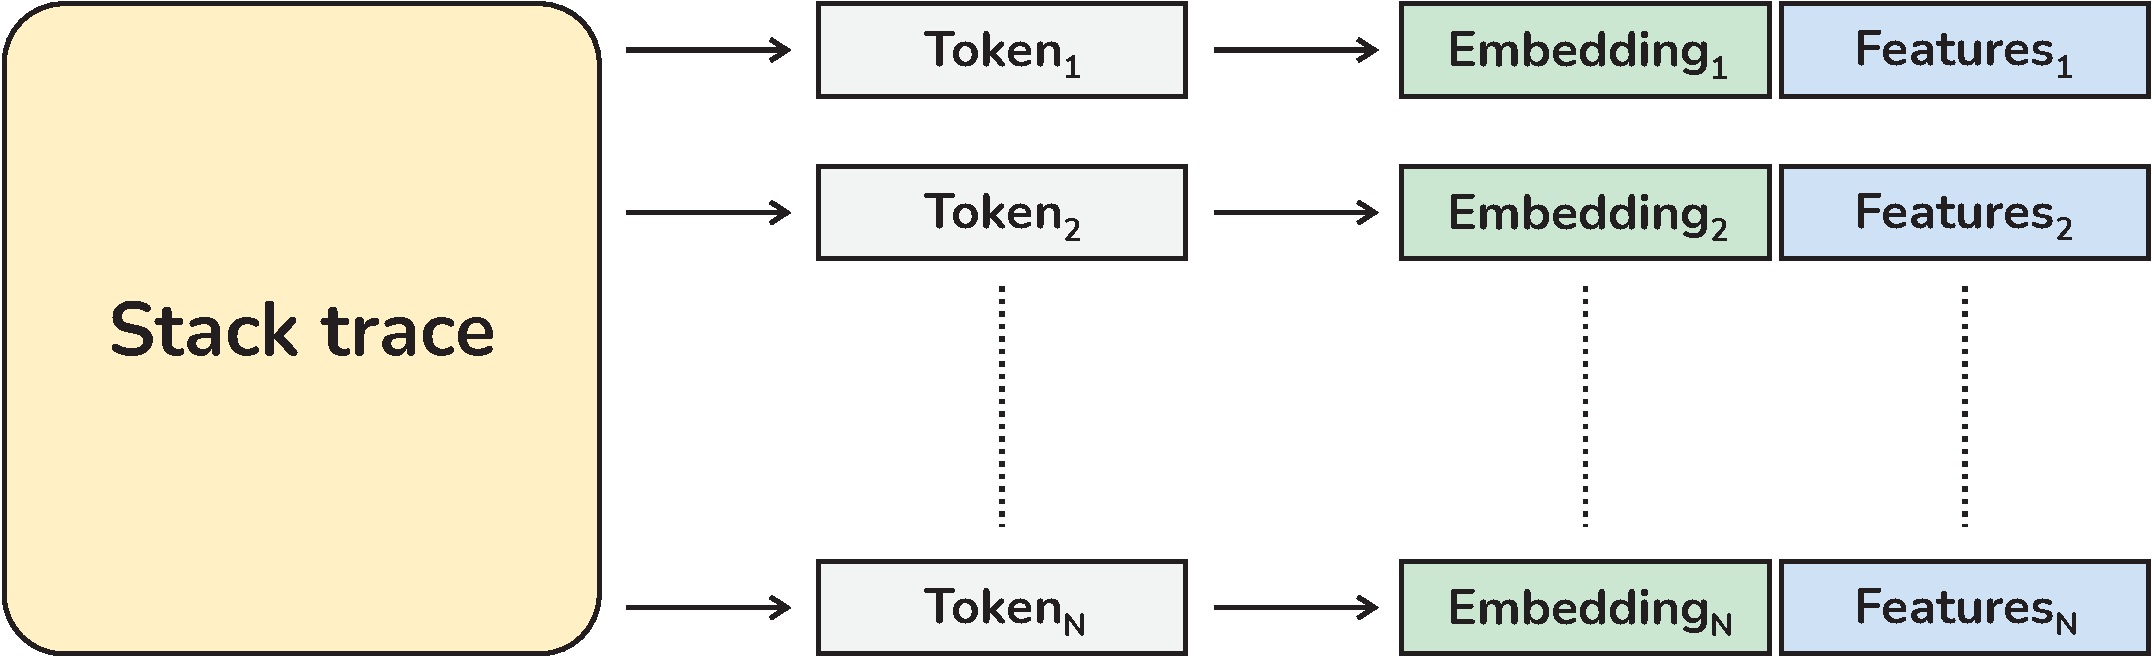
\includegraphics[width=\columnwidth]{figures/03-approach/frame-features.pdf}
        \vspace{-0.4cm}
        \centering
        \caption{The application of the frame-based features.}
        \label{fig:approach-frame-features}
    \end{figure}
    
The features that relate to the entire stack trace can be concatenated to the bug embedding and the developer embedding as presented in \Cref{fig:approach-overall-features}. The resulting vector is the input of the comparison module. 
    
    \begin{figure}[htbp]
        \centering
        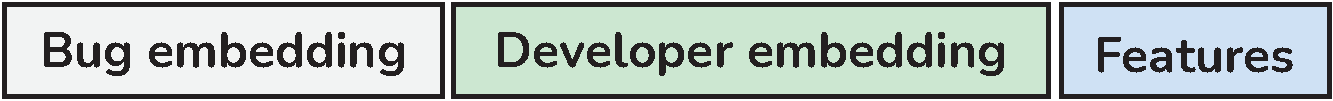
\includegraphics[width=\columnwidth]{figures/03-approach/overall-features.pdf}
        \vspace{-0.4cm}
        \centering
        \caption{The application of the stack-based features.}
        \label{fig:approach-overall-features}
    \end{figure}

We performed feature engineering on the private dataset, trying different combinations of metrics and their normalization methods. We ended up with 15 frame features and 24 stack trace features that worked best in our setting. They are presented in \Cref{table:annot-features}. 
For example, from the first line of the table, we get three different features: a raw value of the minimum distance and two normalizations (by annotation length and by the minimum value).

\secpart{Neural Annotation Processing}
\label{sec:neural-features}

Manual feature engineering is a complex process that requires domain knowledge and expertise. As an alternative, we also propose using another neural network to extract features from annotations automatically.

The idea behind the annotation processing is as follows: each line of an annotation is labelled with a timestamp of its last change. We suggest to represent annotation lines as elements of a time series --- a sequence of values indexed in the chronological order. We propose to use the distance from the current line to the error line (simply subtracting the line numbers) as the values of the time series, and timestamps of the last modification as the corresponding time.
The considered time series is irregular: code lines could be changed at any time. 
Since this is the first work using DL-based annotation processing, we decided to start with simple things first and use the most popular and straightforward solution for irregular time series processing: concatenate the time information to the time series value to form a vector of size 2.

\Cref{fig:approach-annotation-embedding} shows an example of the annotation processing for developer \textit{Mike}, this will be done for each developer and for each stack frame: 

\begin{itemize}
    \item Select lines from the annotation that were edited by Mike.
    \item Sort the lines by time. Each annotation line is mapped to a vector of length 2. The first component of the vector is the distance to the error line $|error\_line - current\_line|$ (in out example, the error line is line 3, highlighted in red). The second component of the vector is the coded line timestamp. In our data, time is measured in milliseconds, therefore we use $\log{(report\_timestamp - line\_timestamp)}$ to account for the order of magnitude.
    \item The sequence of such vectors is processed using the RNN with attention as described in \Cref{sec:vector-representation}. 
\end{itemize}

\begin{figure}[t]
    \centering
    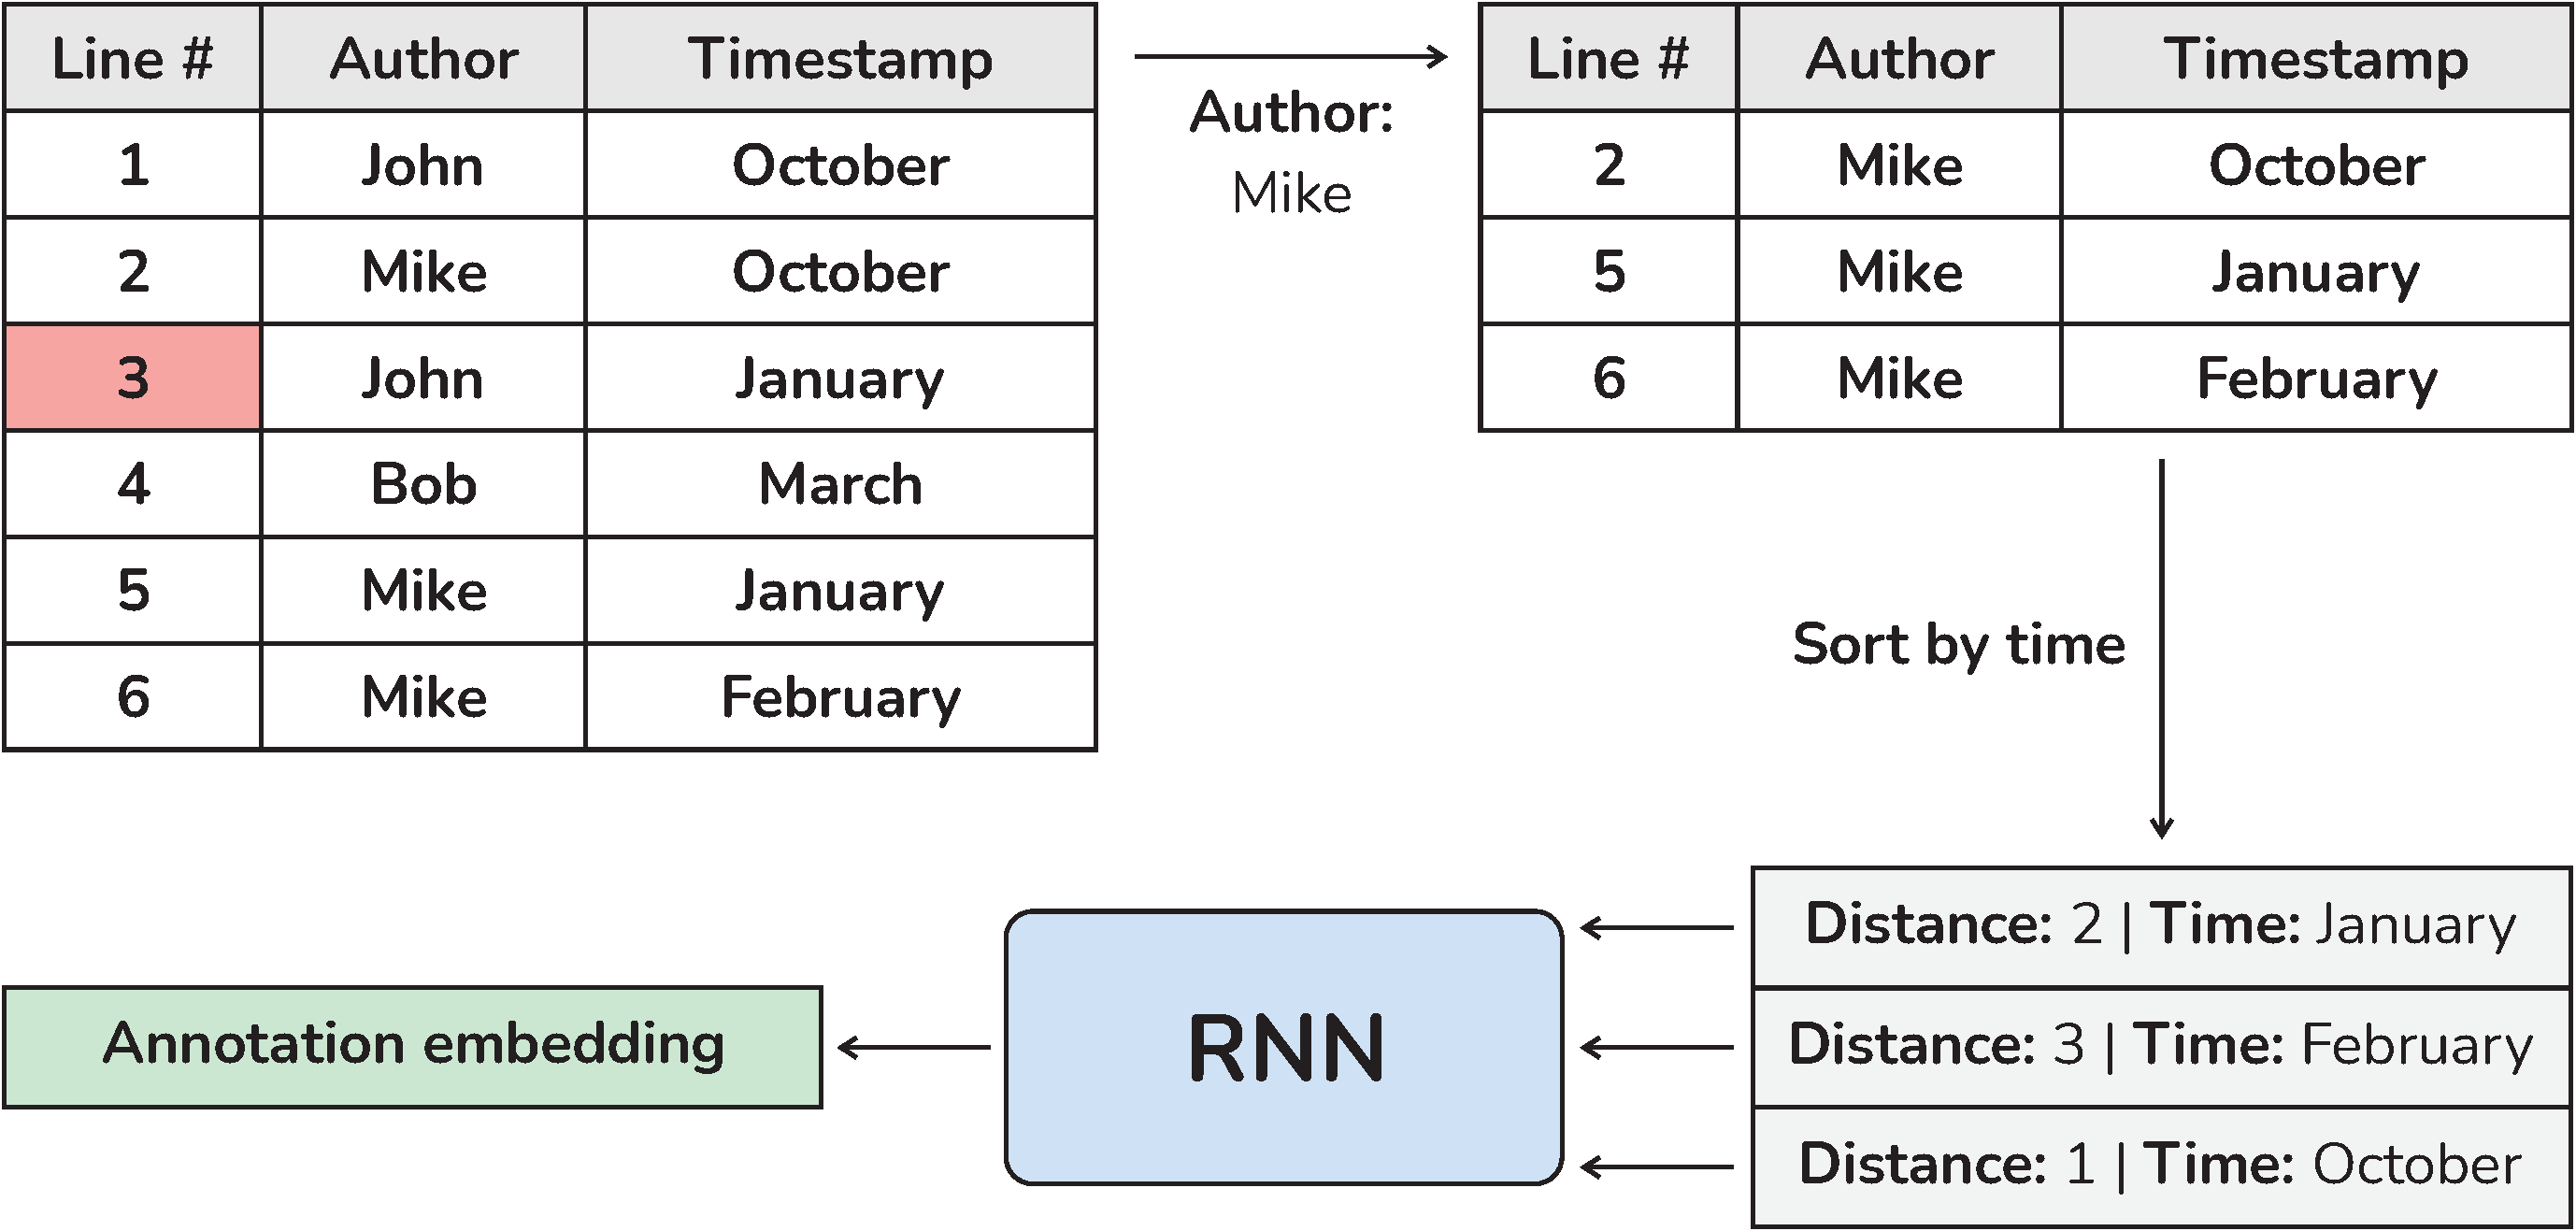
\includegraphics[width=\columnwidth]{figures/03-approach/annotation-embedding.pdf}
    \centering
    \caption{The example processing of an annotation.}
    \label{fig:approach-annotation-embedding}
\end{figure}

The obtained annotation embedding can be used as an alternative to manual features extracted from annotations. 

\secpart{Similarity of Vector Representations}
\label{sec:vector-similarity}
After obtaining the embeddings of the bug and the developer, we feed them into a comparison module. Here, we have applied the approach from the work of Severyn et al.~\cite{Severyn2015LearningTR}, proposing to form the following vector:
\begin{align}
    \mathbf{x}_{join} = [ \mathbf{x}^T_q; x_{sim}; \mathbf{x}^T_d; \mathbf{x}^T_{feat} ],
\end{align}
where $\mathbf{x}_q$, $\mathbf{x}_d$, $\mathbf{x}_{feat}$ stand for the bug embedding, the developer embedding, and additional stack trace features described in Sections \ref{sec:manual-features} and \ref{sec:neural-features}. A scalar value $x_{sim}$ is obtained from $\mathbf{x}^T_q \mathbf{M} \mathbf{x}_d$ with a trainable matrix $\mathbf{M}$, which captures syntactic and semantic aspects between the queries and documents. 

After that, a feed-forward neural network with one hidden layer and ReLU activation function is applied, and the score is obtained which is used to rank developers. 